\documentclass[10pt, xcolor=table]{beamer}
\usepackage{inputenc}
\usepackage{graphicx}
\usepackage {mathtools}
\usetheme{CambridgeUS}
\usecolortheme{dolphin}
\usepackage{booktabs}
\usepackage{lscape}
\usepackage{caption}
\usepackage{tikz}
\usepackage{subcaption}
\usepackage{multicol}
\usepackage{xcolor}
\usepackage{pgfplots}
\usepackage{bm}
\usepackage{multicol}
\usepackage{adjustbox}
\usepackage{multicol}
\usepackage{cleveref}

\newcommand\dc[1]{\textcolor{blue}{#1}}
\setcounter{tocdepth}{3}
\pgfplotsset{compat=1.16}
\usepgfplotslibrary{external} 
\tikzexternalize

\newlength\figureheight
\newlength\figurewidth

\definecolor{myNewColorA}{RGB}{176,179,43}  % Yellow-Green
\definecolor{myNewColorB}{RGB}{42,111,74}   % Green
\definecolor{myNewColorC}{RGB}{52,142,209}  % Blue
\definecolor{myNewColorD}{RGB}{195,36,37}   % Red

\setbeamercolor*{palette primary}{bg=myNewColorC}
\setbeamercolor*{palette secondary}{bg=myNewColorB, fg=white}
\setbeamercolor*{palette tertiary}{bg=myNewColorA, fg=white}
\setbeamercolor*{titlelike}{fg=myNewColorA}
\setbeamercolor*{title}{bg=myNewColorA, fg=white}
\setbeamercolor*{item}{fg=myNewColorA}
\setbeamercolor*{caption name}{fg=myNewColorA}

\usefonttheme{professionalfonts}




\usepackage{natbib}
\usepackage{hyperref}
%------------------------------------------------------------
\titlegraphic{
    \begin{figure}
        \centering
        \begin{subfigure}[l]{0.45\textwidth}
            \centering
            
\includegraphics[width=2.5cm,height=1.5cm]{images/Logo_U.T.P.png}
        \end{subfigure}
        \hfill
        \begin{subfigure}[r]{0.45\textwidth}
            \centering
            
\includegraphics[width=2.5cm,height=2.5cm]{images/logo-maestria-scaled.jpg}
        \end{subfigure}
    \end{figure}
}

\setbeamerfont{title}{size=\Large\bfseries}
\setbeamerfont{subtitle}{size=\small}
\setbeamerfont{author}{size=\small}
\setbeamerfont{institute}{size=\footnotesize}

\title[Universidad Tecnológica de Pereira]{Stochastic Modeling of Multiple Streamflow Time Series in Colombian Based on Gaussian Processes}


 
\author[Julián David Pastrana-Cortés]{%
	\texorpdfstring{
		\begin{tabular}{c}
			\textbf{Author}: Julián David Pastrana-Cortés \\[1.5mm]
			\textbf{Director}: Álvaro Angel Orozco-Gutiérrez \\[1.5mm]
			\textbf{Co-director}: David Augusto Cardenas-Peña \\
		\end{tabular}
	}{Julián David Pastrana-Cortés}
}



\institute[Automatic]{Automatic Research Group}
\date{\today}

\AtBeginSection[]{
  \begin{frame}
    \vfill
    \centering
    \begin{beamercolorbox}[sep=8pt,center,shadow=true,rounded=true]{title}
      \usebeamerfont{title}\insertsectionhead\par%
    \end{beamercolorbox}
    \vfill
  \end{frame}
}

%------------------------------------------------------------

\begin{document}

\frame{\titlepage}
\section{Introduction}
\begin{frame}{Motivation}
	
	Understanding the implications of time series associated with hydrological variables, such as flow rates or reservoir levels, is essential for hydroelectric generation and the planning of other generation systems in Colombia
	
	\begin{figure}
		\centering
		\begin{subfigure}[b]{0.3\textwidth}
			\centering
			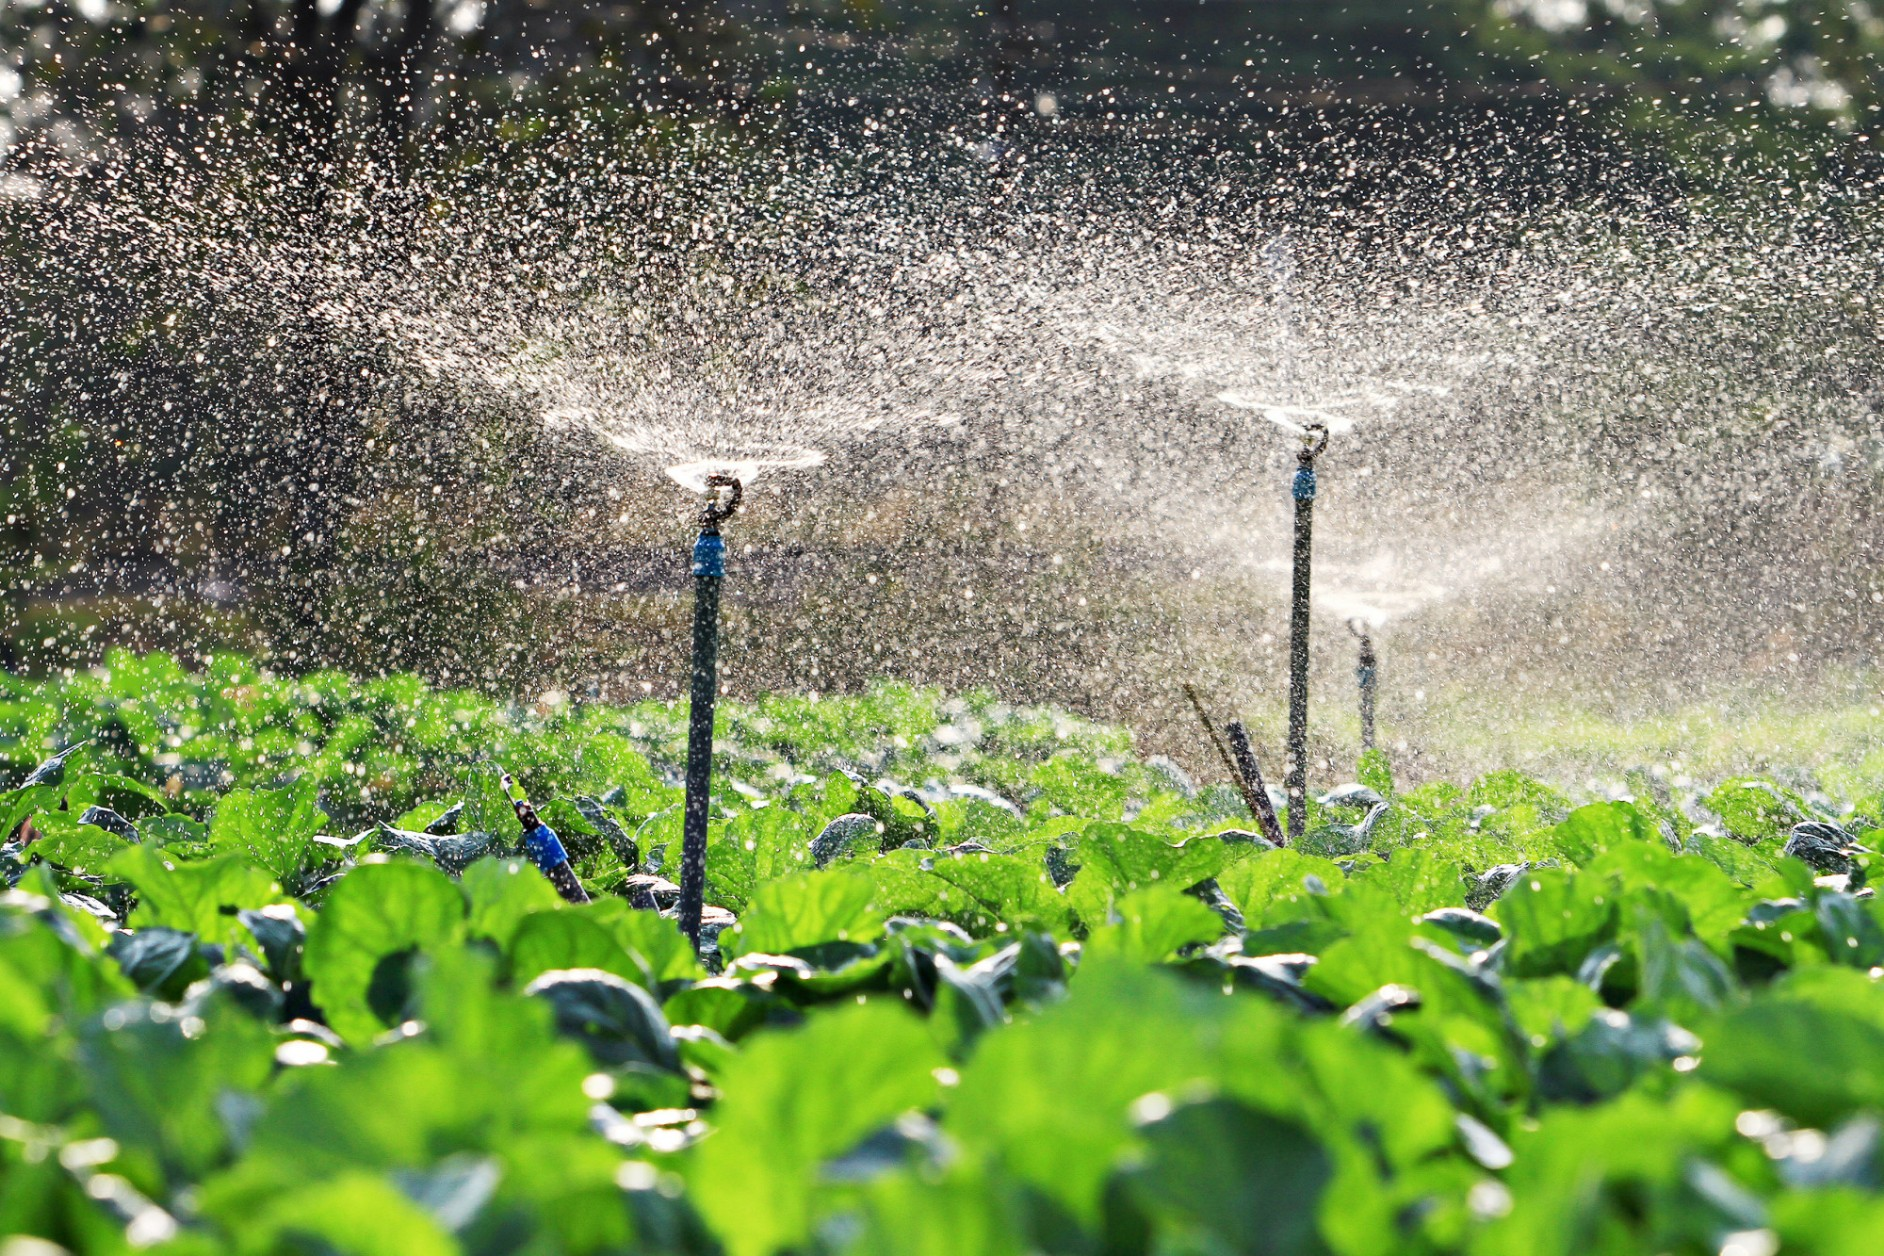
\includegraphics[width=\textwidth, height=4cm]{images/irrigation.jpg}
			\caption{Irrigation}
		\end{subfigure}
		\hfill
		\begin{subfigure}[b]{0.3\textwidth}
			\centering
			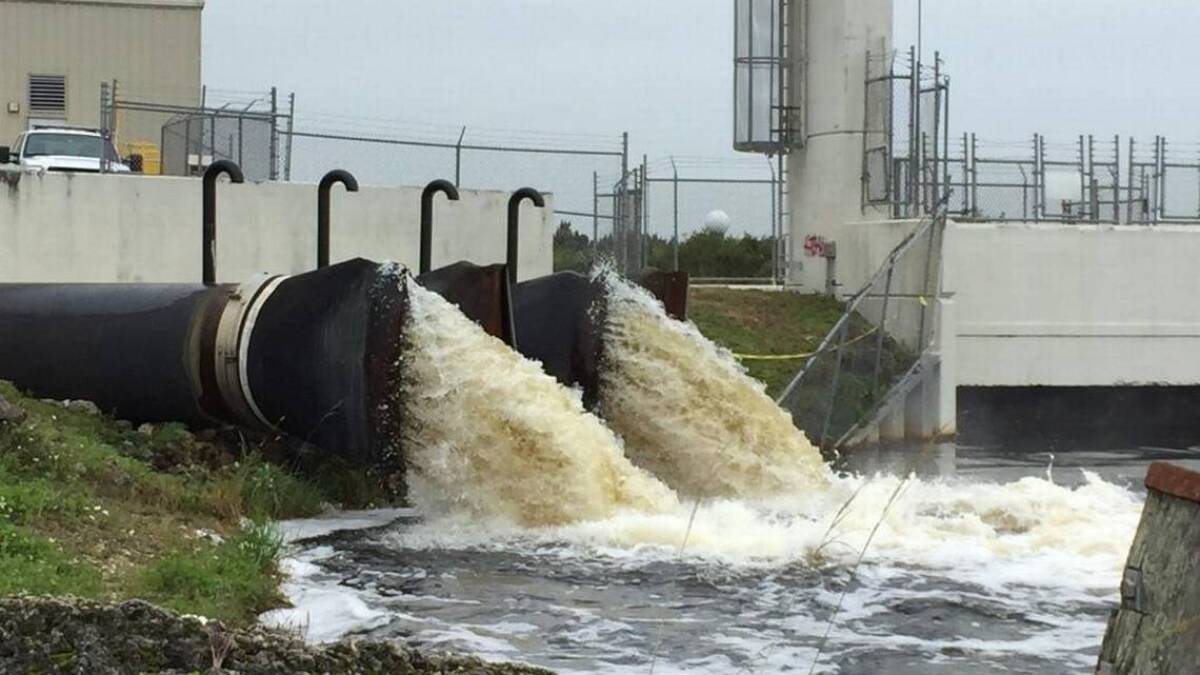
\includegraphics[width=\textwidth, height=4cm]{images/flood_control.jpeg}
			\caption{Flood control}
		\end{subfigure}
		\hfill
		\begin{subfigure}[b]{0.3\textwidth}
			\centering
			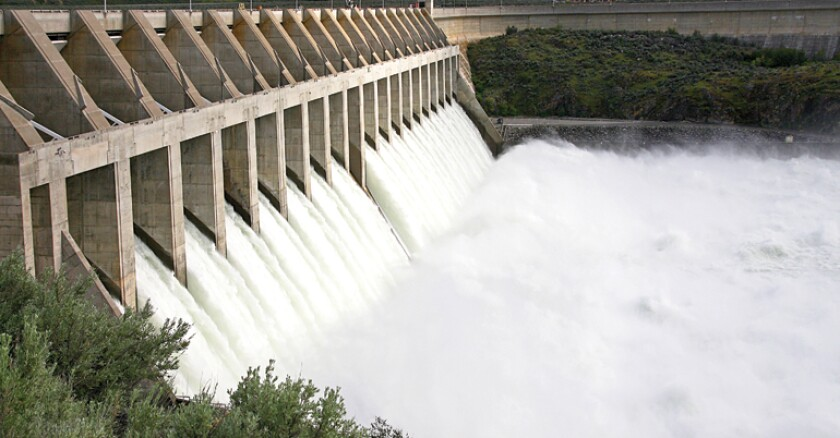
\includegraphics[width=\textwidth, height=4cm]{images/hydro_gen.jpeg}
			\caption{Hydropower generation}
		\end{subfigure}
		
	\end{figure}
\textcolor{myNewColorB}{\textbf{Challenges}}: non-linearities, high stochasticity, and complex water resource patterns.

\end{frame}

\begin{frame}
	\frametitle{The Importance of Hydrological Forecasting}
	
	Understanding hydrological processes has become increasingly critical in the field of natural resource management, anticipation capacity of extreme hydrological events such as droughts and heavy rainfall.
	
	\begin{figure}
		\centering
		\begin{subfigure}[b]{0.45\textwidth}
			\centering
			\includegraphics[width=\textwidth, height=4cm]{images/drought.jpg}
			\caption{Drought Condition}
		\end{subfigure}
		\hfill
		\begin{subfigure}[b]{0.45\textwidth}
			\centering
			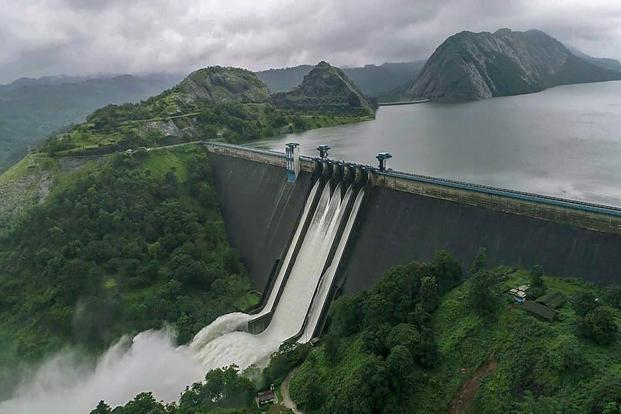
\includegraphics[width=\textwidth, height=4cm]{images/full_dam.jpg}
			\caption{Full Dam}
		\end{subfigure}
	\end{figure}
	
\end{frame}

\begin{frame}{The Proposed Model}
	A Gaussian Process (GP) is a Bayesian non-parametric model that provides not just point predictions but a full probability distribution, capturing uncertainty and enabling confidence intervals in time series forecasting.
	
	\begin{figure}
		\centering
		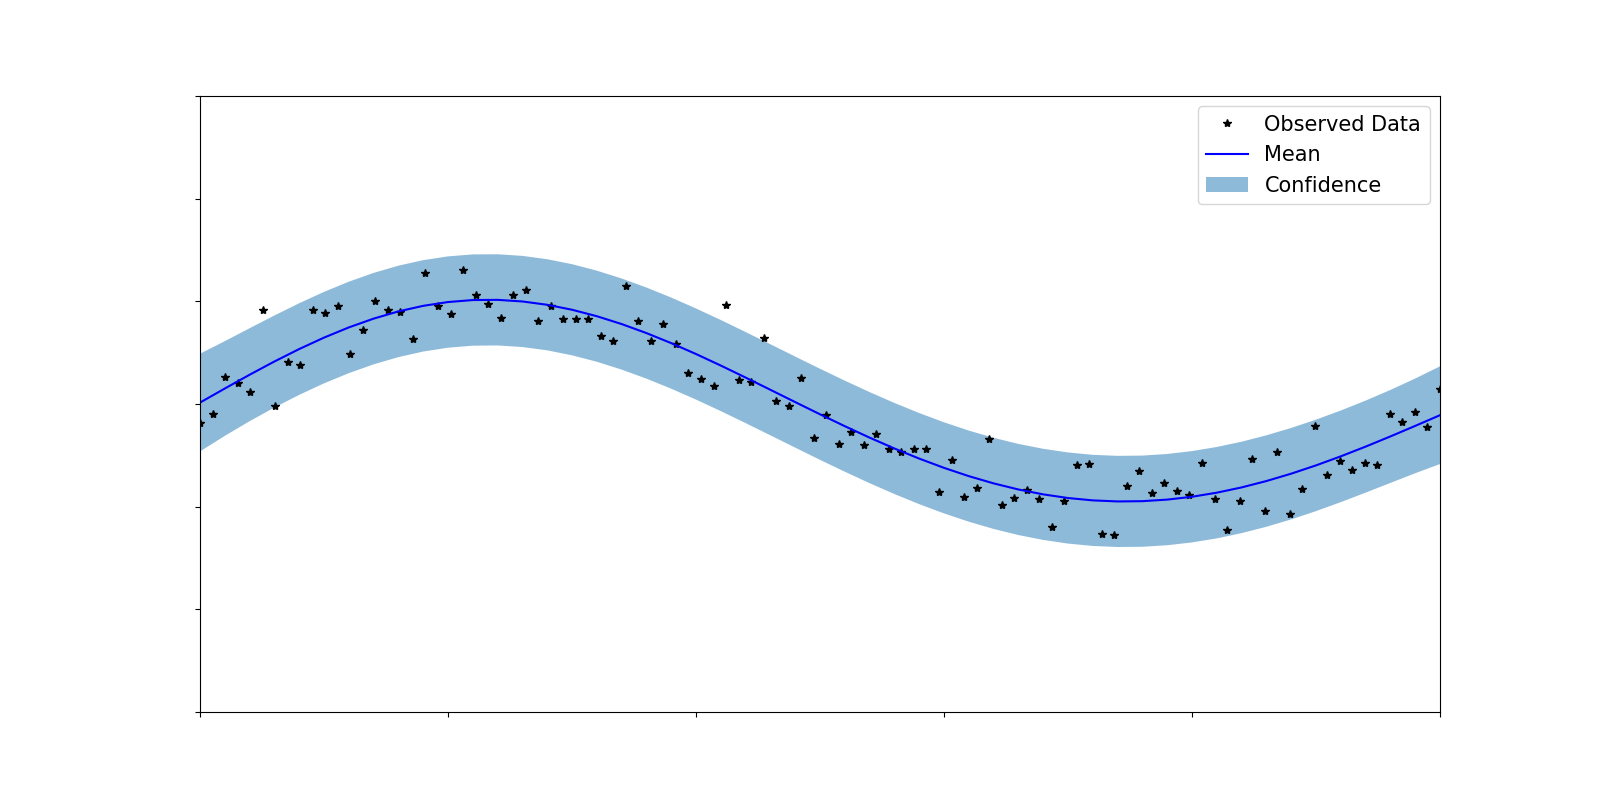
\includegraphics[width=\textwidth]{images/gpr.png}
	\end{figure}
\end{frame}

\section{Objectives}
\begin{frame}{General Objective}
	Develop a stochastic forecasting model for making multiple simultaneous predictions of hydrological time series, taking advantage of cross-correlations among the tasks to improve the performance keeping the scalability in its implementation for the short-term horizon.	
\end{frame}

\begin{frame}{Specific Objectives}
	\begin{itemize}
		\item Develop a model that allows the forecasting of hydrological time series, properly quantifying the uncertainty associated with each value within the prediction horizons.
		\item Design a multi-task forecasting methodology that captures and models cross-correlations between hydrological time series, to improve forecast accuracy within forecast horizons.
		\item Develop a multi-task prediction methodology that handles data constraints across reservoirs while maintaining high forecasting performance as measured by probabilistic metrics.
		
		% \item Develop a scalable multi-task prediction methodology across reservoirs, without compromising regression performance.
	\end{itemize}
\end{frame}

\section{The Dataset}
\begin{frame}{Problem Setting - Part 1}
	Consider a time-series vector of hydrological resources observed across all $D$ outputs at the $n$-th time instant, denoted as $\mathbf{v}_n \in \mathbb{R}^D$. Our model employs the entire sequence of resource vectors from time $n$ back to $n-T+1$ as input to predict the resource vector at the future time step $n+H$. Here, $T$ represents the model order, and $H$ denotes the prediction horizon. 
	
	Consequently, we define the input vector $\mathbf{x}_n$ as follows:
	
	\begin{equation*}
	\mathbf{x}_n = \begin{bmatrix} 
	\mathbf{v}_{n}^\top \\ 
	\mathbf{v}_{n-1}^\top \\ 
	\vdots \\ 
	\mathbf{v}_{n-T+1}^\top 
	\end{bmatrix} \in \mathbb{R}^{DT}
	\end{equation*}
\end{frame}

\begin{frame}{Problem Setting - Part 2}
	The target output vector $\mathbf{y}_n$ is defined as follows:
	
	\begin{equation*}
	\mathbf{y}_n = \mathbf{v}_{n+H}.
	\end{equation*}
	
	This formulation enables the model to leverage historical hydrological data for accurate future predictions. Accordingly, we build a dataset $\mathcal{D} = \{\bm{x}_n, \bm{y}_n\}_{n=1}^N = \{\mathbf{X}, \mathbf{y}\}$ comprising $N$ input--output pairs, where $\bm{x}_n \in \mathcal{X}\subset \mathbb{R}^{DT}$ represents the dimensional input space. The target function is a vector-valued function where $\bm{y}_n \in \mathbb{R}^{D}$ comprises the observations of all outputs (tasks) at the same input $\bm{x}_n$.
\end{frame}

\begin{frame}
	The hydrological forecasting task for validating the proposed model regressors considers time-series streamflow contributions data from 23 Colombian reservoirs.
	\begin{figure}[htbp]
		\centering 
		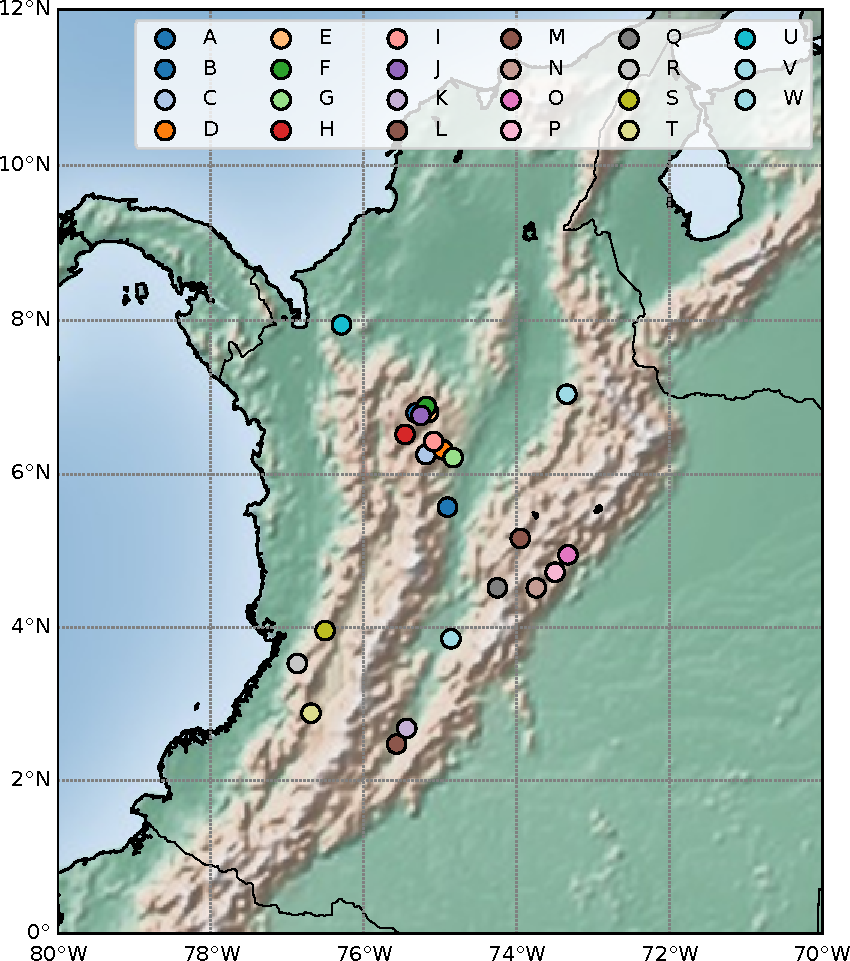
\includegraphics[height=0.5\textwidth]{images/colombiamap.pdf}
		\caption{Reservoir locations in Colombia.}
	\end{figure}
\end{frame}

\begin{frame}
	The dataset was selected due to the strong dependence of time series on weather patterns, which are closely tied to hydropower dispatch operations.
	
	\begin{figure}[htbp]
		\centering
		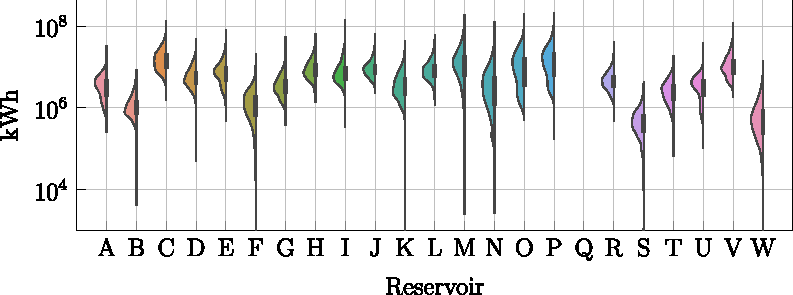
\includegraphics[height=0.25\textwidth]{images/ct_violinplot.pdf}
		\caption{Time-series Violin plot depicting the streamflow contribution for each reservoir within the dataset.}
	\end{figure}	
	
	These streamflow contributions were recorded daily from 1 January 2010 to 28 February 2022. While these contributions represent volumetric values, they are reported in kilowatt-hours (kWh) by the hydroelectric power plants.
\end{frame}



\section[Gaussian Process Regression]{Gaussian Process Regression: Bayesian Non-Parametric Model}
\begin{frame}
	In the GP framework, the dataset $\mathcal{D}$ is used to learn a random mapping function $\bm{f}(\cdot)$, capturing the relationship between $\bm{x}_n$ and $\bm{y}_n$. We define a GP distribution over $\bm{f}(\cdot)$ as:
	\begin{equation}\label{mogp_notation}
	\bm{f}(\bm{x}) \sim  \mathcal{GP}\left(\bm{0},\, \bm{k}(\bm{x}, \bm{x}' \mid \bm{\theta})\right)
	\end{equation}
	where $\bm{f}: \mathcal{X} \rightarrow \mathbb{R}^D$ maps the input space, and $\bm{k}: \mathcal{X} \times \mathcal{X} \rightarrow \mathbb{R}^{D \times D}$ is the cross-covariance matrix function, parameterized by $\bm{\theta}$. Adding i.i.d Gaussian noise $\bm{\epsilon}$ with covariance $\Sigma_\epsilon = \text{diag}\{\sigma^2_{Nd}\}_{d=1}^D$, the model prediction becomes $\bm{y}_n = \bm{f}(\bm{x}_n) + \bm{\epsilon}$.
\end{frame}

\begin{frame}{Joint Distribution}
	Let $\mathbf{X}_* = \{\bm{x}_{n*}\}_{n=1}^{N_*}$ be a set of test points $\bm{x}_{n*} \in \mathcal{X}$ with test output vector $\mathbf{f}_* = [\bm{f}(\bm{x}_1)^\top, \bm{f}(\bm{x}_2)^\top, \cdots, \bm{f}(\bm{x}_{N_*})^\top]^\top \in \mathbb{R}^{N_* D}$. The joint Gaussian distribution over $\mathbf{y}$ and $\mathbf{f}_*$ is given by:
	
	\begin{equation}\label{sogp_prior_matrix}
	\begin{array}{rcl}
	\left[ \begin{array}{c}
	\mathbf{y}\\
	\mathbf{f_*}\\
	\end{array}
	\right]
	\sim
	\mathcal{N} \left(
	\bm{0},
	\left[ \begin{array}{cc}
	\mathbf{K}_y & \mathbf{K}_*\\
	\mathbf{K}_*^\top & \mathbf{K}_{**}\\
	\end{array}
	\right] \right)
	\end{array}
	\end{equation}
	
	Here, $\mathbf{K}_y=\mathbf{K} + \Sigma_\epsilon$ with $\mathbf{K} \in \mathbb{R}^{ND \times ND}$, formed by evaluating the covariance function at all pairs in $\mathbf{X}$. The matrices $\mathbf{K}_{**} \in \mathbb{R}^{N_*D \times N_*D}$ and $\mathbf{K}_{*} \in \mathbb{R}^{ND \times N_*D}$ are formed by evaluating the covariance function across test inputs in $\mathbf{X}_*$ and test-train inputs, respectively.
\end{frame}

\begin{frame}{Posterior Distribution}
	This notation allows for deriving the conditional distribution named posterior as follows:
	
	\begin{equation}\label{sogp_posterior}
	\mathbf{f}_*|\mathbf{X}_*, \mathcal{D} \sim \mathcal{N}(\bar{\mathbf{f}_*},\text{cov}(\mathbf{f}_*))
	\end{equation}
	with
	\begin{equation}\label{sogp_posterior_mean}
	\bar{\mathbf{f}_*} = \mathbf{K}_*^\top \mathbf{K}_y^{-1} \mathbf{y}
	\end{equation}
	\begin{equation}\label{sogp_posterior_cov}
	\text{cov}(\mathbf{f}_*) = \mathbf{K}_{**} -  \mathbf{K}_*^\top \mathbf{K}_y^{-1} \mathbf{K}_*
	\end{equation}
\end{frame}

\begin{frame}{The Marginal Log-likelihood}
	 Furthermore, the prediction performance archived by the conditional distribution depends on the selected parameter set $\bm{\theta}$ and observation noise matrix $\Sigma_\epsilon$. Both parameters are calculated by maximizing the marginal log-likelihood from \Cref{sogp_prior_matrix} where $p(\mathbf{y}) = \mathcal{N}(\mathbf{y} \mid \bm{0}, \mathbf{K}_y)$ as follows:
	\begin{equation}\label{eq:sogp_nlml_opt}
	\begin{aligned}
	\{\bm{\theta}_{\text{opt}}, {\Sigma_\epsilon}_{\text{opt}}\} &= \underset{\bm{\theta}, \Sigma_\epsilon}{\arg\max} \quad \ln p(\mathbf{y})\\
	&= \underset{\bm{\theta}, \Sigma_\epsilon}{\arg\min} \quad \frac{1}{2} \mathbf{y}^\top \mathbf{K}_y^{-1} \mathbf{y} + \frac{1}{2} \ln \mid \mathbf{K}_y \mid + \frac{ND}{2} \ln 2\pi
	\end{aligned}
	\end{equation}
	
	The main challenge is their computational complexity of $\mathcal{O}(N^3D^3)$ and storage demand of $\mathcal{O}(N^2D^2)$ due to inverting the matrix $\mathbf{K}_y$.
\end{frame}

\begin{frame}{Variational Inference}
	A common approach to reduce GP complexity, consists of the introduction of a reduced set of $M \ll N$ inducing point locations, denoted by $Z$, containing vectors $\mathbf{z} \in \mathcal{X}$, and an inducing variable vector $\mathbf{u} = [\bm{f}(\bm{z}_1)^\top, \bm{f}(\bm{z}_2)^\top, \cdots, \bm{f}(\bm{z}_{M})^\top]^\top \in \mathbb{R}^{M D}$. This approach leads to the following extended joint distribution:
	\begin{equation}
	\begin{array}{rcl}
	\left[ \begin{array}{c}
	\mathbf{u}\\
	\mathbf{f}\\
	\end{array}
	\right]
	\sim
	\mathcal{N} \left(
	\begin{array}{c}
	\mathbf{0}\\
	\end{array},
	\left[ \begin{array}{cc}
	\mathbf{K}_{uu} & \mathbf{K}_{uf}\\
	\mathbf{K}_{uf}^\top & \mathbf{K}\\
	\end{array}
	\right] \right)
	\end{array}
	\end{equation}
	
	Here, $\mathbf{K}_{uu} \in \mathbb{R}^{MD \times MD}$ and $\mathbf{K}_{uf} \in \mathbb{R}^{MD \times ND}$ represent the block covariance matrices evaluated at the inducing point pairs and between the inducing points and training inputs, respectively. We call this model the Sparse Variational Gaussian Process (SVGP). 
	
\end{frame}

\begin{frame}{The Variational Distribution}
	From the above, the conditional distribution is given by:
	\begin{equation}
	p(\mathbf{f} \mid \mathbf{u}) = \mathcal{N}\left( \mathbf{f} \mid \mathbf{K}_{uf}^\top \mathbf{K}_{uu}^{-1} \mathbf{u}, \mathbf{K} - \mathbf{K}_{uf}^\top \mathbf{K}_{uu}^{-1} \mathbf{K}_{uf}\right),
	\end{equation}
	and the prior for the inducing variables is:
	\begin{equation}
	p(\mathbf{u}) = \mathcal{N}\left(\mathbf{u} \mid \mathbf{0}, \mathbf{K}_{uu} \right).
	\end{equation}
	The joint posterior distribution over the latent variable $\mathbf{f}$ and inducing variable $\mathbf{u}$ is:
	\begin{equation}
	p(\mathbf{f}, \mathbf{u} \mid \mathbf{y}) = p(\mathbf{f} \mid \mathbf{u}) p(\mathbf{u} \mid \mathbf{y}).
	\end{equation}
	However, computing $p(\mathbf{u} \mid \mathbf{y})$ is typically intractable, so we use variational inference to approximate the posterior with a variational distribution $q(\mathbf{u}) = \mathcal{N}\left( \mathbf{u} \mid \boldsymbol{\mu}, \boldsymbol{S} \right)$, where $\boldsymbol{\mu} \in \mathbb{R}^{MD}$ and $\boldsymbol{S} \in \mathbb{R}^{MD \times MD}$. The approximate joint posterior then becomes:
	\begin{equation}\label{eq:so_join_posterior}
	p(\mathbf{f}, \mathbf{u} \mid \mathbf{y}) \approx q(\mathbf{f}, \mathbf{u}) = p(\mathbf{f} \mid \mathbf{u}) q(\mathbf{u}).
	\end{equation}
	
\end{frame}

\begin{frame}{ELBO}
	Accordingly, the approximation of the posterior distribution consists of estimating the variational parameters $\boldsymbol{\mu}$ and $\boldsymbol{S}$, performed by maximizing an evidence lower bound (ELBO). Such ELBO is obtained from the log marginal likelihood:
	\begin{equation}
	\ln p(\mathbf{y}) \geq \int \int q(\mathbf{f}, \mathbf{u}) \ln \frac{p(\mathbf{y} \mid \mathbf{f}) p(\mathbf{f}\mid \mathbf{u}) p(\mathbf{u})}{q(\mathbf{f}, \mathbf{u})} d\mathbf{f} d\mathbf{u} = \mathcal{L}
	\end{equation}
	resulting from the Jensen's inequality. We can rewrite the previous expression to derive the following:
	\begin{equation}
	\mathcal{L} = \mathbb{E}_{q(\mathbf{f})}\{\ln p(\mathbf{y} \mid \mathbf{f})\} - \text{KL}\{q(\mathbf{u})\parallel p(\mathbf{u})\}
	\end{equation}
	Here, $\text{KL}$ represents the Kullback--Leibler divergence between the Gaussian-shaped distributions.
\end{frame}

\begin{frame}{ELBO}
	With the i.i.d assumption, the likelihood function $p(\mathbf{y} \mid \mathbf{f})$ can be factorized over observations and outputs:
	\begin{equation}
	p(\mathbf{y} \mid \mathbf{f}) = \prod_{d=1}^D\prod_{n=1}^N p(y_{dn} \mid f_{d}(\mathbf{x}_n)),
	\end{equation}
	where $f_{d}(\mathbf{x}_n)$ represents the latent function value for the $d$-th output at the $n$-th input, and $y_{dn}$ is the corresponding label. The lower bound can then be expressed as:
	\begin{equation}\label{eq:sogp_elbo}
	\mathcal{L} = \sum_{d=1}^D\sum_{n=1}^N \mathbb{E}_{q(f_{d}(\mathbf{x}_n))}\{\ln p(y_{dn} \mid f_{d}(\mathbf{x}_n))\} - \sum_{d=1}^D \text{KL}\{q(\mathbf{u}_d)\parallel p(\mathbf{u}_d)\}.
	\end{equation}
	
	The summation over $D$ and $N$ facilitates training through a mini-batch fashion.
\end{frame}

\begin{frame}{Posterior and Predictive Distribution}
	We define the variational distribution for $\mathbf{f}$ as:
	\begin{align}
	q(\mathbf{f}) &:= \int p(\mathbf{f} \mid \mathbf{u}) q(\mathbf{u}) d\mathbf{u} \nonumber \\
	&= \mathcal{N}\left(\mathbf{f} \mid \mathbf{K}_{uf}^\top \mathbf{K}_{uu}^{-1} \boldsymbol{\mu}, \mathbf{K} + \mathbf{K}_{uf}^\top \mathbf{K}_{uu}^{-1}(\mathbf{S} - \mathbf{K}_{uu})\mathbf{K}_{uu}^{-1}\mathbf{K}_{uf} \right).
	\end{align}
	
	This approach reduces complexity to $\mathcal{O}(NM^2D^3)$, as $\mathbf{K}_{uu}$ is smaller than $\mathbf{K}_{y}$. For predictions at new points $\mathbf{x}_*$, we compute:
	\begin{equation}
	p(\mathbf{f}_* \mid \mathbf{y}) \approx q(\mathbf{f}_*) = \int p(\mathbf{f}_* \mid \mathbf{u}) q(\mathbf{u}) d \mathbf{u},
	\end{equation}
	and adding Gaussian noise $\Sigma_\epsilon$ to the latent posterior $\mathbf{f}_* \mid \mathbf{y}$.
\end{frame}

\begin{frame}{Model Setup}
	The proposed approach factorizes the GP scalar covariance function into two kernels: $k_{\mathcal{X}}$, which models input correlations via relative distances, and $k_{D}$, which models task pair-wise correlations as follows:
	
	\begin{align}
	k\left((\bm{x}, d), (\bm{x}', d') \mid \bm{\theta}\right) &= k_{\mathcal{X}}\left(\bm{x}, \bm{x}' \mid \bm{\Theta}_d \right) k_{D}\left(d, d' \mid \sigma_d \right), \\
	k_{\mathcal{X}}\left(\bm{x}, \bm{x}' \mid \bm{\Theta}_d \right) &= \text{exp}\left(-\frac{1}{2}(\bm{x} - \bm{x}')^\top \bm{\Theta}_d^{-2} (\bm{x} - \bm{x}')\right), \\
	k_{D}\left(d, d' \mid \sigma^2_d \right) &= \sigma^2_d ~ \delta_{d, d'},
	\end{align}
	
	where $\delta_{d, d'}$ is the Kronecker delta, $\sigma^2_d$ is the output scale for task $d$, and $\bm{\Theta}_d$ is a diagonal matrix of lengthscale factors. The input kernel $k_{\mathcal{X}}$ uses a squared-exponential function, ensuring smooth data mapping. The task kernel $k_{D}$ avoids modeling task correlations directly, reducing complexity to $\mathcal{O}(N M^2 D)$. Despite not modeling task correlations explicitly, the autoregressive inputs and shared inducing points still enable exploration of task dependencies.
	
\end{frame}

\begin{frame}
	To evaluate our model's performance, we use three metrics: Mean Squared Error (MSE), Mean Standardized Log Loss (MSLL), and Continuous Ranked Probability Score (CRPS).
	
	MSE measures the average squared difference between the observed outcome $y_{dn}$ and the predicted expectation $\mathbb{E}\{y_{dn*}\}$:
	\begin{equation}\label{eq:mse}
	\text{MSE} = \frac{1}{DN_{*}} \sum_{d=1}^{D} \sum_{n=1}^{N_*} (y_{dn} - \mathbb{E}\{y_{dn*}\})^2
	\end{equation}
	MSLL assesses the quality of probabilistic predictions by considering the log-likelihood of observed values:
	\begin{equation}
	\text{MSLL} = \frac{1}{2DN_{*}} \sum_{d=1}^{D} \sum_{n=1}^{N_*} \left( \frac{(y_{dn} - \mathbb{E}\{y_{dn*}\})^2}{\text{var}\{y_{dn*}\}} - \frac{(y_{dn} - \mu_d)^2}{\sigma_d^2} + \ln \left(\frac{\text{var}\{y_{dn*}\}}{\sigma_d^2}\right) \right)
	\end{equation}
	CRPS evaluates probabilistic predictions by comparing the predicted CDF $\Phi(y_{dn})$ with the empirical CDF:
	\begin{equation}
	\text{CRPS} = \frac{1}{DN_*} \sum_{d=1}^{D} \sum_{n=1}^{N_*} \sqrt{\text{var}\{y_{dn*}\}} \left(\beta_{dn} \left( 2\Phi\left(\beta_{dn}\right) - 1 \right) + 2\phi\left(\beta_{dn}\right) - \frac{1}{\sqrt{\pi}} \right)
	\end{equation}
	where $\beta_{dn} = \frac{y_{dn} - \mathbb{E}\{y_{dn*}\}}{\sqrt{\text{var}\{y_{dn*}\}}}$.
\end{frame}


\end{document}



